\documentclass{article}

\usepackage{physics} % Handy shortcuts like \pdv, \dd and much more
\usepackage{geometry} % smaller margins, can be adjusted if given arguments
\usepackage{siunitx} % the \si environment for units
\usepackage{mathtools} % The dcases environment, prettier than just cases
\usepackage{tikz} % For drawing picures
\usepackage{wrapfig} % Wrapping text around figures

\title{Exercise x - TFY4345 Classical Mechanics}
\date{2020}

\begin{document}
    \maketitle

    \section{Elastic scattering in laboratory coordinates}
    (Corse book p 115-120 and lecture notes chapter 4)\\
    Consider the relation between laboratory and center-of-mass (CM) scattering angles
    \begin{equation}
        \cos(\vartheta) = \frac{\cos(\Theta) + \rho}{\sqrt{1 + 2\rho \cos(\Theta) + \rho^2}},
    \end{equation}
    and the resulting expression for cross sections 
    \begin{equation}
        \sigma'(\vartheta) = \sigma (\Theta) \frac{(1 + 2\rho \cos(\Theta) + \rho^2)^{3/2}}{1 + \rho \cos(\Theta)}
    \end{equation}
    Let us assume that we have two particles with equal masses, $m_1 = m_2$, which scatter elastically ($\rho = m_1/m_2 = 1$). The first particle is the incoming particle, while the latter is initially at rest. Derive the connection between the scattering angles ($\vartheta$ in the lab frame, $\Theta$ in the CM frame), and cross sections ($sigma(\vartheta)$ in the lab frame, $\sigma'(\Theta)$ in the CM frame) based on the equations above. Furthermore, what is the ration of the kinetic energy of particle q before and after the scattering ($E_1 / E_2$)
    \\
    \\
    Hint: you will need this general trigonometric relation with the scattering angles:
    \begin{equation}
        \cos(\alpha/2) = \sqrt{\frac{1 + \cos(\alpha)}{2}}
    \end{equation}

    \section{Rotating system in cylindrical coordinates.}
    Write down Lagrange's and Hamilton's equations in cylindrical coordinates, $(q_1, q_2, q_3) = (r, \theta, z)$ for a particle with mass $m$ in an potential $V = V(q_    i)$.
    \\
    \\
    Hint: you do not need to do the Legendre transformation $H = \sum_i p_i \dot q_i - L$. Which assumptions gives a much easier equation for the Hamiltonian? Are they satisfied here? (See Goldstein p. 338-339 3rd ed.)

    \newpage
    \section{Centrifugal force and gravitation}

    \begin{wrapfigure}{2}{0.5\textwidth}        
        \begin{tikzpicture}
            \def\R{2}:
            \draw (0, 0) node[](O) {} circle (\R);
            \draw[-stealth] (O) -- (10:\R) node[midway, above]{$R$};
            \draw[line width = 1mm] (\R, 0) -- (3*\R, 0) node[midway, above]{$L, \lambda$};
            \draw[-stealth] (0, \R) -- (0, 1.5*\R) node[midway, left]{$\omega$};
            \draw[-stealth] (0, 1.1*\R) ++(-30:0.1*\R) arc (0:180:0.1*\R);
        \end{tikzpicture}
    \end{wrapfigure}

    A rigid, strong rod with uniform mass density $\lambda$ hangs upright in a stationary position over a fixed point at the equator, without being suspended at any point. The rod follows the rotation of the earth. Thus, the effects of gravitation equals that of the centrifugal term. What is the length of the rod? Use that the radius of the earth is $R = 6400 \si{km}$.
    \\
    \\
    Hint: You need to consider two integrals. Either calculate the angular velocity of the earth yourself, or look at the lecture notes.
    \\
    \\

    \section{Coriolis effect on a falling particle}

    \begin{wrapfigure}{2}{0.4\textwidth}
        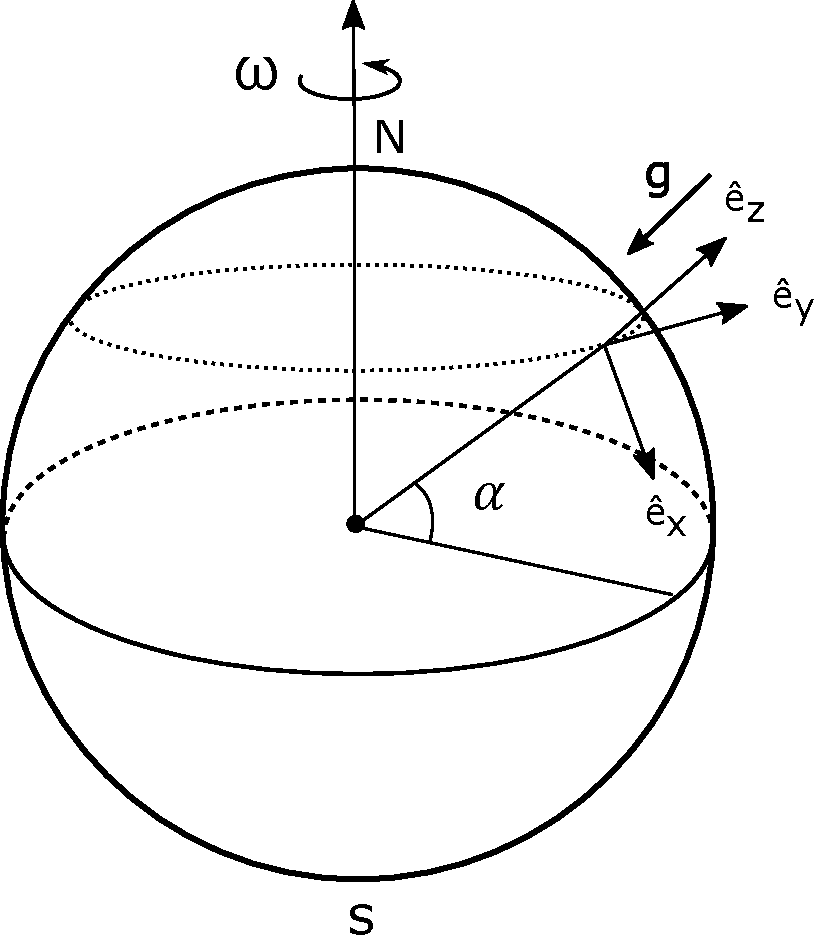
\includegraphics[width=0.4\textwidth]{figures/exercise_6_4_earth.pdf}        
    \end{wrapfigure}

    Find the horizontal deflection from the straight line caused by the Coriolis force on a particle falling freely in the gravitational field of the earth, from a height $h$ above the surface. What is the direction of the deflection?
    \\
    \\
    Hint: You can safely neglect the $x$- and $y$- components of the velocity when finding the determinant for the cross problem. Why is this?
    \\
    \\
    Historical note: The direction of the deflection was already predicted by Isaac Newton (1697) and confirmed experimentally by Robert Hooke and several others. The most careful measurements were preformed by F. Reich (1831), who dropped pellets down a mine shaft $188 \si{m}$ deep, and observed a mean deflection of $28 \si{mm}$. This value is smaller than the prediction by theory (as you have done) due to air resistance effects.
    \\
    \\
    Physical note: If one shoots the particle upwards initially, so that it reaches the altitude $h$ before falling down, the final deflection on the ground will be in the revers direction (see exam December 2017).

\end{document}
